% !TeX root = ../thuthesis-example.tex

\begin{translation}
\label{cha:translation}

\title{一日建成罗马}
\author{Sameer Agarwal, Yasutaka Furukawa, Noah Snavely, Ian Simon, Brian Curless, Steven M. Seitz, Richard Szeliski}
\maketitle
\tableofcontents

\textbf{摘要:}我们提出了一个系统,可以从庞大无序的照片集合中重建三维几何,比如通过在照片分享网站上搜索给定的城市(如罗马)而找到的图片。我们的系统建立在一系列新的分布式计算机视觉算法上,用于图像匹配和三维重建,旨在最大限度地提高流程中每个阶段的并行性,并根据问题的规模和可用的计算量进行调整。我们的实验结果表明,现在有可能在不到一天的时间里重建超过十万张图像的城市规模的图像集合。

\section{简介}
曾几何时,摄影是很大程度上归功于个人的付出。在过去,摄影师会把一个瞬间拍下来,与一些朋友和家人分享,也许会把几百张照片储存在一个相册里。数字摄影的出现,以及\href{https://www.flickr.com}{Flickr.com}等照片分享网站的增长,给摄影和相册的使用带来了翻天覆地的变化。今天,一张在网上分享的照片可能会被数百万人看到。

因此,我们现在有机会通过世界各地的人每天对其城市和地标数以万计的拍摄,来获得一个巨大的、不断增长的照片集。例如,在Flickr网站上搜索“罗马”这个词会得到近300万张照片,这些照片代表了一个越来越完整的城市摄影记录,包括了每一个受欢迎的地点:建筑外观、室内、喷泉、雕塑、绘画和咖啡店等。事实上,人们在罗马发现的任何有趣的东西都是在无数的光照和天气条件下从数千个视角捕捉到的。例如,特莱维喷泉出现在了5万多张照片中。

在这样的一个照片集合中,罗马城能够在多大程度上被重建?原则上来讲,Flickr上的罗马照片是3D建模研究的理想数据集,因为它们从各个视角精确地捕捉了城市的每一个亮点。然而,从这样的集合中提取高质量的3D模型是具有挑战性的,原因有以下几点。首先,这些照片是非结构化的,它们没有按照特定的顺序拍摄,我们无法控制相机视点的分布。其次,它们来自于数千名摄影师之手,是未经校正的照片,我们对相机设置知之甚少。第三,问题的规模是巨大的,以前的方法只处理数百或最多几千张照片,而我们的规模比它们高三个数量级。第四,算法必须快——我们要在一天之内重建整个城市,这样就有可能多次重复这个算法来重建世界上所有重要的文化中心。

建立精确的城市三维模型是一个具有广泛应用价值的问题。在政府领域,城市模型对于城市规划和可视化至关重要。它们对历史学、考古学、地理学和计算机图形学等广泛的学术学科同样重要。数字城市模型也是地图和可视化应用的核心,比如谷歌地球和必应地图,以及gps导航系统。在不久的将来,这些模型可以实现增强现实功能,在你的手机或其它屏幕上识别和标注物体。这种功能可以让游客找到它们感兴趣的位置,驾驶方向,并在一个新的环境中确定自己的方位。

城市规模的三维重建以前也有探索\cite{antone2002scalable,fruh2004automated,pollefeys2008detailed, zebedin2008fusion}。然而,现有的大型系统操作的数据来自一个结构化的来源,例如,由调查飞机拍摄的航空照片或由移动的车辆拍摄的街道图像。这些系统依赖于使用相同参数的相机以固定采样率拍摄的照片,并且通常利用其他传感器,如GPS和惯性导航单元来极大地简化计算。从网页上获取的图像没有这些简化特征。因此,我们工作的一个关键焦点是开发新的3D计算机视觉技术,使其能够更灵活地被应用在更丰富、更大型、更无约束的图像集合中。

我们解决这个问题的方法建立在近年来计算机视觉方面取得的进展(包括我们自己最近在Photo Tourism\cite{snavely2006photo}和Photosynth方面的工作),并借鉴了计算机科学的许多其他领域,包括分布式系统、算法、信息检索和科学计算。

\section{运动恢复结构}
我们如何从一组图像中恢复三维几何结构?一个基本的挑战是照片是三维世界的二维投影。反推这个投影是困难的,因为我们失去了每个点在图像的深度。作为人类,我们可以闭上一只眼睛来体验这个问题,并注意到我们的深度知觉减弱了。幸运的是,我们有两只眼睛,我们的大脑可以通过我们感知的两幅图像之间的关联点来估算深度。这给了我们一些希望,从多个场景的照片,我们可以恢复该场景的形状。

考虑图\ref{appendix-fig-1}(a)中显示的三个多维数据集图像。我们不知道这些图像是在哪里拍摄的,我们也不知道它们描绘的是一个特定的形状(在这个例子中,是一个立方体)。然而,假设我们确实知道在图像中看到的立方体的角,即3D角的2D投影,是对应的,即我们知道具有相同颜色的2D点对应于相同的3D点。这种对应为我们提供了一组强大的摄像机和点的3D几何约束。一种表述这些约束的方法是,给定场景几何(用3D点表示)和摄像机几何(每个摄像机的3D位置和方向),我们可以通过透视投影方程预测每个点的2D投影在每个图像中的位置;然后我们可以将这些投影与原始测量值进行比较。
\begin{figure}
	\centering
	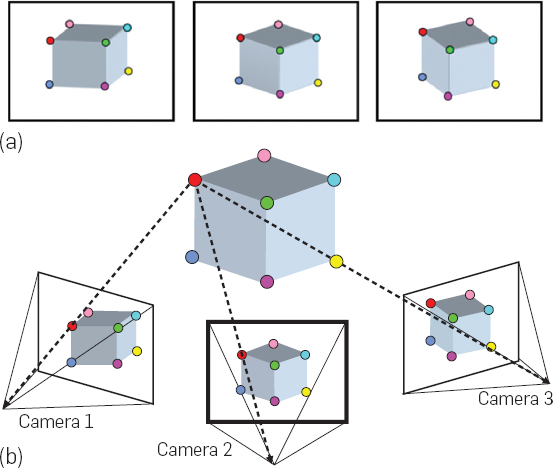
\includegraphics[width=9cm]{appendix-fig-1}
	\caption[]{(a)一个立方体的三幅图像,从未知的视角。角上的彩色编码点显示了这些图像中某些2D点之间的已知对应关系;每一组相同颜色的点是同一3D点的投影。(b)上图所示的三维点(较大的彩色点)和相机的候选重建。集合中的每个图像都有一个关联的位置和方向。这种重建与观测到的二维投影基本一致;当红色的3D点投影到每个图像(用虚线表示)时,预测的投影与观察到的投影很接近。在相机3的情况下,投影略有偏差;由此产生的残差称为重投影误差,是我们要尽量减小的。}
	\label{appendix-fig-1}
\end{figure}

具体来说,假设$X_i,i=1,...,8$表示立方体的三个角的三维位置,$R_j$,$c_j$和$f_j$,$j=1,2,3$表示三个摄像机的方位、位置和焦距。那么如果$x_{ij}$是点$X_i$在图像$j$上的像素,我们可以把成像方程写成
\begin{equation}
	\label{eq1}
	x_{ij}=f_j\prod(R_j(X_i-c_j))
\end{equation}
其中投影函数为$(x,y,z)=(x/z,y/z)$。运动结构(Structure from Motion,SfM)问题是从观测$x_{ij}$中推断$Xi$,$R_j$,$c_j$和$f_j$。

这样做的标准方法是将问题表述为最小化总平方重投影误差的优化问题:

\begin{equation}
	\label{eq2}
	\mathop{\arg\min}\limits_{X_i,R_j,c_j,f_j}\sum_{i-j}\left\| x_{ij}-f_j\prod\left(R_j(X_i-c_j)\right) \right\|^2
\end{equation}

上式中,$i-j$表示点$X_i$在图像$j$中可见。图\ref{appendix-fig-1}为实例重建,说明重投影误差。虽然这个问题很容易解决,式\ref{eq2}通常是一个复杂的非线性最小二乘问题,有许多局部最小值,在大的场景中有数百万个参数。第5节描述了我们用于大规模解决式\ref{eq2}的各种技术。

\section{对应关系问题}
\label{sec-3}
在上面的立方体例子中,我们假设输入图像之间有一组2D对应。但在现实中,这些对应并没有给出,必须从图像中估计。如何能自动完成这一项任务?这就是对应关系问题。

为了解决两幅图像之间的对应问题,我们可以考虑第一幅图像中的每个图像块,然后在第二幅图像中找到最相似的图像块。然而,这种算法很快就遇到了问题。首先,许多图像补丁可能很难匹配。例如,对于一个晴朗的蓝天的图像块而言,这个问题就变得非常具有挑战性,因为它看起来和天空的其他任何一块相似,也就是说它是不明显的。第二,如果第二个图像是在一天的不同时间或使用不同的缩放级别拍摄的,会发生什么?

过去的10年见证了算法的发展,用于检测拍摄图像中最独特、可重复的特征。这样的特征检测器不仅将图像表示减少到更易于管理的规模,而且还为匹配提供更加鲁棒的特征,对多种图像变换具有不变性。其中最成功的检测器之一是SIFT(尺度不变特征变换)\cite{lowe2004distinctive}。

一旦我们检测到图像中的特征,我们可以通过寻找相似的特征来匹配图像对中的特征。虽然穷尽匹配两幅图像之间的所有特征代价高昂,但使用近似最近邻搜索已经获得了很好的结果\cite{snavely2006photo};本文使用了ANN库\cite{arya1998optimal}。对于每对图像,其中一张图像的特征被插入到$k$-d树中,另一张图像的特征被用作查询。对于每个查询,如果ANN返回的最近邻居离下一个最近邻居足够远,则它们就被认为是一对匹配\cite{lowe2004distinctive}。

尽管SIFT特征具有尺度不变性和对外观变化的鲁棒性,但它是局部的,不包含关于图像或其他特征在图像中的位置的任何全局信息。因此,基于SIFT特征的特征匹配仍然容易出错。然而,由于我们假设我们处理的是刚性场景,在匹配特征的位置上有很强的几何约束,这些约束可以用来排除误匹配。特别地,当两个针孔摄像机对一个刚性场景进行成像时,存在一个$3\times 3$的本质矩阵$F$,使图像$j$和图像$k$中对应的点$x_{ij}$和$x_{ik}$(以齐次坐标表示)满足\cite{andrew2001multiple}
\begin{equation}
	\label{eq3}
	x_{ij}^TFx_{ik}=0
\end{equation}

施加这一约束的一种常见方法是使用贪婪随机算法生成适当选择的$F$的随机估计值,并选择在所有的匹配点对中拟合最好的,例如最满足式\ref{eq3}的约束的。这种算法被称为随机抽样一致(RANSAC)\cite{fischler1981random},被用于解决许多计算机视觉问题。

\section{城市规模匹配}
\label{sec-4}
第3节描述了如何找到一对图像之间的对应关系。然而,我们的任务是在一个拥有数万或数十万张图像的大型集合中寻找对应关系。考虑这个图像匹配问题的一种方法是作为一个图估计问题,在这个问题中我们得到了一组定点,对应与集合中的图像,我们想要发现连接这些顶点的边的集合。在这个图中,一条边连接一对图像,当且仅当它们能看到场景的相同部分,并且之间有足够数量的特征匹配。我们称这个图为匹配图。

确定匹配图中所有边的一种简单方法是执行所有$O(n^2)$个图像匹配;然而,对于大型集合,这是不实际的。对于一组10万张图像,这意味着50亿个成对比较,如果500个核心以每核每秒10对图像的速度运行,那么需要11.5天才能匹配,再加上在机器之间传输图像和特征数据所需的时间。此外,即使我们能够完成所有这些成对匹配,也会浪费计算的精力,因为绝大多数的图像对无法匹配,也就是说,图是稀疏的对于整个城市的图像都是这样。

因此,我们的系统采用了一种多轮方案进行替代:在每一轮中,我们在匹配图中提取一组边,然后通过特征匹配来验证其中的每条边。如果我们找到的特征数量超过某一阈值,我们就保留这条边,否则就丢弃它。因此,问题减少为制定一种快速预测两幅图像何时匹配的方法。我们使用两种方法来生成提取边:整体图像相似度和查询扩展。

\subsection{整体图像相似度}
\label{sec-4-1}
一个自然的想法是提出一个简洁的表示来计算两个图像的总体相似度,然后使用这个度量提取边进行测试。

对于文本文档,有许多技术可以快速比较两个文档的内容。一种常见的方法是将每个文档表示为一个加权词频向量\cite{jones1972statistical};这两个向量之间的距离可以很好地预测相应文档之间的相似性。

受文本分析工作的启发,计算机视觉研究人员最近开始将类似的技术应用于视觉对象识别,并取得了巨大的成功\cite{chum2007total, nister2006scalable, schindler2007city, sivic2003video}。其基本思想是在一组照片中提取SIFT特征,并将它们聚为“视觉词汇”。通过将图像作为由这些视觉词组成的文档来处理,我们可以利用文档检索的机制来有效地匹配大型照片数据集。我们使用一种快速的树状结构方法来关联视觉词与图像特征\cite{nister2006scalable}。每幅图片都被表示为视觉词的稀疏直方图,我们使用著名的“词频-逆向文件频率”(TFIDF)方法对其进行加权\cite{jones1972statistical};我们通过取它们的内积来比较这两个直方图。对于每个图像,我们确定$k_1+k_2$个最相似的图像,并验证前$k_1$个,这是第一轮配对的建议。

在这个阶段,我们有一个稀疏连接的匹配图。为了获得最全面的重建,我们需要一个连通分量尽可能少的图。为此,我们进一步利用整个图像相似度的建议来尝试连接该图中的各种连通分量。对于每个图像,我们考虑整个图像相似性建议的下$k_2$个图像,并验证那些跨越两个不同连接连通分量的对。我们仅对具有2个或更多连通分量中的图像执行此操作\footnote{我们在所有实验中使用的是$k_1=k_2=10$}。

\subsection{查询扩展}
\label{sec-4-2}
在基于整个图像相似性执行两轮匹配之后,我们得到了一个稀疏匹配图,但是这个图通常不够密集,无法可靠地产生良好的重建。为了解决这个问题,我们使用了来自文本和文档检索研究查询扩展的另一个想法\cite{chum2007total}。

在其原始形式中,查询扩展采用一组与用户查询匹配的文档,然后使用这些初始结果再次查询,从而扩展初始查询。最终结果是这两个查询的组合。如果我们在文档集(包括查询)上定义一个图,其中相似的文档由一条边连接,那么查询扩展等效于查找查询顶点两步内的所有顶点。

在我们的系统中,对于匹配图中的每个顶点$j$,如果顶点$i$和$k$与$j$相连,我们建议$i$和$k$也相连,并验证边$(i,k)$。这个过程可以重复固定次数或直到匹配图收敛。

\subsection{分布式实现}
\label{sec-4-3}
我们现在考虑上述想法的分布式实现。我们的匹配系统分为三个不同的阶段:(1)预处理(第\ref{sec-4-3-1}节),(2)验证(第\ref{sec-4-3-2}节)和(3)轨迹生成(第\ref{sec-4-3-3}节)。该系统运行在一组计算机(节点)上,其中一个节点被指定为主节点,负责作业调度决策。
\subsubsection{预处理和特征提取}
\label{sec-4-3-1}
我们假设图像在中央存储上可用,它们从那里以固定大小的块按需分发到集群节点。每个节点将其图像下采样到固定大小并提取SIFT特征。这会自动执行负载平衡,更强大的节点会接收更多要处理的图像。这是唯一需要中央文件服务器的阶段;系统的其余部分在不使用任何共享存储的情况下运行。

在这个阶段结束时,图像集(连同它们的特征)被划分为不相交的集,每个节点一个。

\subsubsection{验证和详细匹配}
\label{sec-4-3-2}
下一步是提出和验证(通过特征匹配)候选图像对,如第\ref{sec-3}节所述。

对于前两轮匹配,我们使用整个图像相似度(第\ref{sec-4-1}节),对于接下来的四轮,我们使用查询扩展(第\ref{sec-4-2}节)。

如果我们把图像对应的TFIDF向量看作是一个巨大矩阵$T$的行,那么评估整个图像相似度的过程就等价于评估外积$S=TT'$。集群中的每个节点评估与其图像对应的行块,选择每行中的前$k_1+k_2$个条目并将它们报告给主节点。查询扩展是一种简单且足够便宜的操作,我们让主节点生成这些建议。

如果图像都位于一台机器上,验证每个提议的对将是一个简单的问题,即遍历提议集并执行SIFT匹配,也许要注意验证的顺序以最小化磁盘I/O。然而,在我们的例子中,图像和特征分布在整个集群中。要求节点匹配图像对$(i,j)$可能需要它从集群的其他两个节点获取图像特征。由于网络传输速度和本地磁盘传输之间的巨大差异,以及为三个节点创建工作,这是不可取的。因此,候选边缘验证应该以尊重数据局部性的方式分布在整个网络中。

我们尝试了许多方法,结果令人惊讶。最初,我们尝试在执行任何验证之前优化网络传输。在这个设置中,一旦主节点知道所有需要验证的图像对,它就会构建另一个连接共享图像的图像对的图。使用MeTiS\cite{karypis1998fast},该图被划分为与计算节点一样多的部分。然后通过解决线性分配问题将分区与计算节点匹配,该问题最小化将所需文件发送到每个节点所需的网络传输数量。

该算法适用于小问题,但不适用于大问题。我们假设验证每对图像花费相同的恒定时间是错误的;一些节点提前完成并空闲长达一个小时。

我们的第二个想法是将图过度分割成小块,然后根据需要将它们打包到节点。当一个节点请求一个工作块时,它被分配到需要最少网络传输的工作块。这种策略实现了更好的负载平衡,但随着问题规模的增长,我们需要分区的图变得非常庞大,分区本身成为一个瓶颈。

给出最佳结果的方法是使用简单的贪心装箱算法,其中每个箱子表示发送到节点的作业集。主节点维护每个节点上的图像列表。当一个节点请求工作时,它会遍历可用图像对的列表,如果它们不需要任何网络传输,则将它们添加到箱子中,直到箱子已满或没有更多图像对要添加。然后它选择一个图像(特征向量列表)传输到节点,选择允许它向箱子添加最大数量的图像对的图像。重复此过程,直到垃圾箱已满。该算法的一个缺点是它可能需要对所有剩余的图像对进行多次扫描:对于大型问题,这可能是一个瓶颈。一个简单的解决方案是只考虑固定大小的图像对子集进行调度。这种窗口化方法在实践中效果很好,我们的实验使用了这种方法。

\subsubsection{跟踪生成}
\label{sec-4-3-3}
到目前为止,我们一次只比较了两个图像。但是,当一个3D点在两个以上的图像中可见并且与该点对应的特征已经在这些图像中匹配时,我们需要将这些特征组合在一起,以便几何估计算法可以从所有特征中估计出单个3D点.我们将与单个3D点对应的一组特征称为特征轨迹(图\ref{appendix-fig-2});匹配过程的最后一步是组合所有成对匹配信息以生成跨图像的一致轨迹。
\begin{figure}
	\centering
	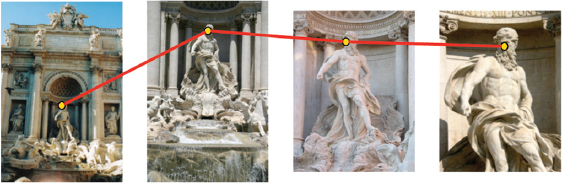
\includegraphics[width=14cm]{appendix-fig-2}
	\caption[]{一条轨道对应于Oceanus中央雕像(希腊神话中环绕世界的河流的化身)面上的一个点。}
	\label{appendix-fig-2}
\end{figure}

轨迹生成问题可以表述为在图中寻找连通分量的问题,其中顶点是所有图像中的特征,边连接匹配特征。由于匹配信息本地存储在计算匹配的计算节点上,因此轨迹生成过程是分布式的并分两个阶段进行。首先,每个节点从其本地匹配数据生成轨迹。这些数据在主节点收集,然后通过网络广播到所有节点。其次,为每个节点分配匹配图的一个连通分量可以独立于所有其他分量进行处理),并将该分量的轨迹拼接在一起。

\section{城市规模的SfM}
生成轨迹后,下一步是在匹配图的每个连通分量上使用SfM算法来恢复每个轨迹的相机姿势和3D位置。

直接求解方程\ref{eq2}是一个困难的非线性优化问题。大多数用于无序照片集合的SfM系统都是增量式的,从一个小的重建开始,然后一次增加一些图像,对新点进行三角测量,并进行一轮或多轮非线性最小二乘优化(称为光束平差法\cite{triggs1999bundle})以最小化重投影错误。重复此过程,直到无法添加更多图像。然而,由于我们收集的规模,一次对所有照片运行这种增量方法是不切实际的。

为了解决这个问题,我们观察到互联网照片集本质上是多余的。许多照片是从附近的视点(例如,斗兽场的正面)拍摄的,处理所有这些照片不一定会增加重建工作。因此,最好找到并重建捕获场景基本几何形状的最小照片子集(在\citet{snavely2008skeletal}中称为骨架集)。一旦重建了该子集,就可以通过估计每个相机相对于与该图像匹配的已知3D点的姿态,一步将剩余图像添加到重建中。这个过程导致性能的一个数量级或更多的改进。

将SfM问题简化为骨架集后,重建过程中的主要瓶颈是使用束调整的式(\ref{eq2})解决方案。Levenberg Marquardt(LM)是解决束调整问题的首选算法;LM每次迭代中的关键计算瓶颈是对称正定线性系统的解,称为正规方程组。

我们开发了新的高性能束调整软件,根据问题的大小,在截断或精确步长LM算法之间进行选择。在第一种情况下,使用预条件共轭梯度法来近似求解正规方程。在第二种情况下,使用CHOLMOD\cite{chen2008algorithm},是一种用于计算Cholesky分解的稀疏直接方法。第一种算法每次迭代的时间复杂度较低,但使用了更多的LM迭代,而第二种算法以每次迭代更多的时间和内存为代价收敛得更快。与最先进的方法相比,生成的代码使用的内存要少得多,并且运行速度快了一个数量级。运行时间和内存节省取决于所涉及的线性系统的稀疏性\cite{agarwal2010bundle}。

\section{多视图立体化}
SfM恢复相机姿势和3D点。然而,重建的3D点通常是稀疏的,仅包含与照片匹配良好的独特图像特征。3D重建的下一阶段是使用多视图立体化(MVS)算法获取注册图像并恢复密集且准确的模型。

MVS算法恢复3D几何信息的方式与我们的视觉系统通过融合两个视图来感知深度的方式非常相似。在MVS设置中,我们可能有许多图像看到相同的点,并且可能用于深度估计。图\ref{appendix-fig-3}说明了基本算法如何估计单个像素的深度值。为了恢复密集模型,我们估计每个图像中每个像素的深度,然后将生成的3D点合并到单个模型中。
\begin{figure}
	\centering
	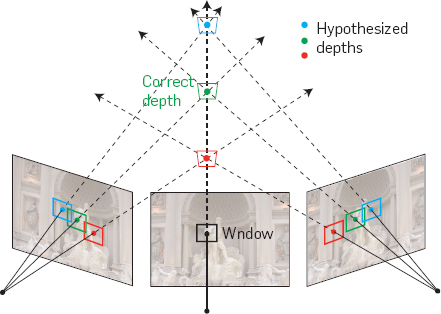
\includegraphics[width=10cm]{appendix-fig-3}
	\caption[]{一种标准的基于窗口的多视图立体算法。给定一个像素和它周围的图像窗口,我们假设沿着它的视线有有限数量的深度。在每个深度,窗口被投影到其他图像中,并评估这些图像投影的纹理之间的一致性。在真实深度(以绿色突出显示)处,一致性得分处于最大值。}
	\label{appendix-fig-3}
\end{figure}

对于城市规模的MVS重建,由于内存消耗过高,照片数量远远超出任何标准MVS算法可以同时处理的数量。因此,关键任务是将照片分组为少量可管理大小的集群,每个集群都可以用来很好地重建场景的一部分。

具体来说,如果我们将SfM点视为密集MVS重建的稀疏代理,我们需要一个聚类使得
\begin{enumerate}
	\item 每个SfM点都可以从集群中的足够多的图像中看到。
	\item 集群的总数很小。
	\item 每个集群的大小都被限制在低于某个阈值,这由机器的内存限制决定。
\end{enumerate}

由此产生的聚类问题是一个受约束的离散优化问题(有关算法细节,请参见\citet{furukawa2010towards})。

聚类后,我们使用MVS算法独立求解每个聚类内的场景几何,然后组合结果\cite{furukawa2010towards}。这种策略不仅可以执行重建,而且可以直接在多个处理器上并行执行此操作。

\section{实验}
我们展示了在从Flickr下载的三个城市规模数据集上运行我们的系统的结果:杜布罗夫尼克、罗马和威尼斯。

SfM实验在具有双四核处理器的62个节点的集群上运行,在具有1GB/s以太网接口的专用网络上运行。每个节点有32GB的RAM和1TB的本地硬盘空间,使用Microsoft Windows Server 2008 64位操作系统。为了将图像编码为TFIDF向量,我们使用了一组由20,000张罗马图像创建的视觉词。用于创建视觉词词汇的图像未用于任何实验。

图\ref{appendix-fig-4}显示了这些数据集最大连通分量的重建。由于篇幅原因,这里只展示了一个结果样本。完整的结果发布在\href{http://grail.cs.washington.edu/rome}{http://grail.cs.washington.edu/rome}。

对于整个图像相似性建议,前$k_1=10$用于第一个验证阶段,接下来的$k_2=10$用于第二个连通分量匹配阶段。进行了四轮查询扩展。在所有情况下,进行的比赛数量与验证的比赛数量的比率在四轮后开始下降。表\ref{appendix-tab-1}总结了三个数据集的统计数据。
\begin{table}
	\centering
	\caption{三个城市的匹配和SfM统计}
	\label{appendix-tab-1}
	\resizebox{\textwidth}{!}{
		\begin{tabular}{ccccccccc}
			\hline
			\textbf{}        & \textbf{}       & \textbf{}      & \textbf{}           & \textbf{}               & \textbf{}            & \multicolumn{3}{c}{\textbf{Time (h)}}                     \\ \cline{7-9} 
			\textbf{Dataset} & \textbf{Images} & \textbf{Cores} & \textbf{Registered} & \textbf{Pairs verified} & \textbf{Pairs found} & \textbf{Matching} & \textbf{Skeletal sets} & \textbf{SfM} \\ \hline
			Dubrovnik        & 57,845          & 352            & 11,868              & 2,658.264               & 498,982              & 5                 & 1                      & 16.5         \\
			Rome             & 150,000         & 496            & 36,658              & 8,825,256               & 2,712,301            & 13                & 1                      & 7            \\
			Venice           & 250,000         & 496            & 47,925              & 35,465,029              & 6,119.207            & 27                & 21.5                   & 16.5         \\ \hline
	\end{tabular}}
\end{table}

表\ref{appendix-tab-1}中的SfM时序数有一些解释。令人惊讶的是,在杜布罗夫尼克上运行SfM花费的时间比在罗马多得多,而且几乎与威尼斯相同,两者都是更大的数据集。原因在于数据集的结构。罗马和威尼斯场景本质上是地标的集合,它们大多具有简单的几何形状和可见性结构。另一方面,杜布罗夫尼克最大的连通分量捕捉了整个老城区。由于其复杂的可见性和广泛变化的观点,重建杜布罗夫尼克是一个复杂得多的SfM问题。这反映在与表\ref{appendix-tab-2}中显示的最大连通分量相关的骨架集的大小中。
\begin{table}
	\centering
	\begin{threeparttable}[c]
		\caption{三个数据集中最大连通分量的重建统计}
		\label{appendix-tab-2}
		\begin{tabular}{ccccc}
			\hline
			\textbf{Data set}     & \textbf{CC1\tnote{a}}     & \textbf{CC2\tnote{b}}     & \textbf{Skeletal set}    & \textbf{Reconstructed\tnote{c}}    \\ \hline
			Dubrovnik             & 6,076            & 4,619            & 977                      & 4,585                     \\
			Rome                  & 7,518            & 2,106            & 254                      & 2,097                     \\
			Venice                & 20,542           & 14,079           & 1,801                    & 13,699                    \\ \hline
		\end{tabular}
		\begin{tablenotes}
			\item [a] CC1指匹配后最大连通分量的大小 
			\item [b] CC2是提取骨架集后最大连通分量的大小
			\item [c] 最后一列指最终重建中的图像数量 
		\end{tablenotes}
	\end{threeparttable}
\end{table}

图\ref{appendix-fig-4}还显示了在我们的匹配和SfM系统生成的城市规模重建上运行我们的MVS\cite{furukawa2010towards}的结果。图\ref{appendix-fig-4}显示了圣彼得大教堂(罗马)、罗马斗兽场(罗马)、杜布罗夫尼克和圣马可广场(威尼斯)的MVS重建(呈现为彩色点),而表\ref{appendix-tab-3}提供了时间和大小统计数据。
\begin{table}
	\centering
	\caption{四个视图簇的 MVS 重建统计数据}
	\label{appendix-tab-3}
	\resizebox{\textwidth}{!}{
		\begin{tabular}{ccccccc}
			\hline
			\textbf{}            & \textbf{}       & \textbf{}                   & \textbf{}         & \multicolumn{3}{c}{\textbf{Time (min)}}                             \\ \cline{5-7} 
			\textbf{Landmark}    & \textbf{Images} & \textbf{Images in clusters} & \textbf{Clusters} & \textbf{MVS points} & \textbf{Clustering} & \textbf{Reconstruction} \\ \hline
			St. Peter's Basilica & 1,275           & 333                         & 4                 & 5,107,847           & 1.3                 & 94.2                    \\
			Colosseum            & 1,167           & 528                         & 7                 & 5,747,083           & 1.5                 & 59.2                    \\
			Dubrovnik            & 6,304           & 2,628                       & 28                & 14,051,331          & 21.1                & 221.4                   \\
			San Marco Square     & 13,709          & 5,917                       & 67                & 27,707,825          & 39.3                & 176.3                   \\ \hline
	\end{tabular}}
\end{table}

最大的数据集San Marco Square包含14,000个输入图像,这些图像被处理成67个集群,并在不到3小时的时间内产生了2800万个表面点。虽然我们的系统成功地为这些非常大的场景重建了密集且高质量的3D点,但我们的模型在某些地方包含孔洞。例如,图像覆盖率较差的屋顶,以及表面通常不清晰可见的地平面。另一方面,在有很多图像的地方,重建质量非常高,如图\ref{appendix-fig-4}中的特写所示。

\begin{figure}
	\centering
	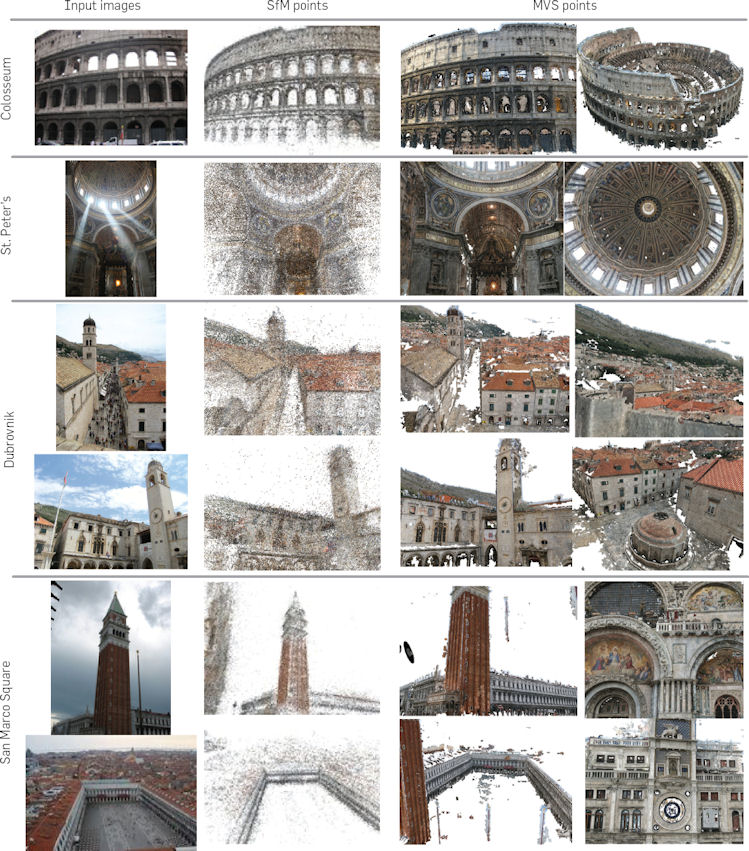
\includegraphics[width=14.5cm]{appendix-fig-4}
	\caption[]{从左到右为:样本输入图像、运动重建的结构和多视图立体重建。}
	\label{appendix-fig-4}
\end{figure}

\section{讨论}
在\href{Flickr.com}{Flickr.com}上搜索关键字“罗马”会产生超过400万张图片。我们的目标是能够在24小时内从这些照片中尽可能多地重建城市。我们目前的系统离这个目标大约有一个数量级的距离。自从这项工作最初发表以来,Frahm等人。已经构建了一个系统,该系统使用GPU的大规模并行性在单个工作站上进行城市规模的重建\cite{frahm2010building}。

在我们的系统中,轨迹生成、骨架集和重建算法都在连通分量的级别上运行。这意味着最大的少数连通分量完全支配了这些阶段。我们目前正在探索将所有这三个步骤并行化的方法,特别强调SfM系统。

当前系统的另一个问题是它会产生一组断开的重建。如果图像带有地理标签/GPS信息,我们的系统可以尝试对重建进行地理定位。然而,这些信息经常是不正确的、嘈杂的或缺失的。

匹配系统的运行时性能关键取决于验证作业在网络上的分布情况。图像在集群节点上的初始分布促进了这一点。根据用户名和图像的Flickr ID存储图像的早期决定意味着同一用户拍摄的大多数图像最终会出现在同一个集群节点上。查看匹配图,事实证明(事后很自然地)用户自己的照片在他们之间有很高的匹配概率。拍照者的ID只是与这些图像相关联的一种元数据。更复杂的策略将利用与图像关联的所有文本标签和地理标签来预测哪些图像可能匹配并相应地分发数据。

最后,我们的系统在设计时考虑了批量操作。一个更具挑战性的问题是使系统成为增量式的。

\textbf{致谢:}

这项工作得到了SPAWAR、NSF grant IIS-0811878、海军研究办公室、华盛顿大学动画研究实验室和 Microsoft的部分支持。 我们感谢 Microsoft Research慷慨地提供对他们的HPC集群和Szymon Rusinkiewicz的Qsplat软件的访问。作者还要感谢与Steven Gribble、Aaron Kimball、Drew Steedly和David Nister的讨论。

	
% 书面翻译的参考文献
\bibliographystyle{plain}
\bibliography{ref/appendix}

% 书面翻译对应的原文索引
\begin{translation-index}
	\nocite{agarwal2011building}
	\bibliographystyle{unsrtnat}
	\bibliography{ref/appendix}
\end{translation-index}

\end{translation}